\documentclass[journal, a4paper]{IEEEtran}

\usepackage{cite}      
\usepackage{graphicx}
\usepackage{url}
\usepackage{amsmath}
\usepackage{float}
\usepackage{caption}
\usepackage{subcaption}

\begin{document}

\title{RANZCR CLiP - An image classification approach }
\author{Matteo Carollo \and Paolo Sofia}
\markboth{Digital Health and Bioinformatic Engineering - Medical Imaging  Course 2020-2021}{}
\maketitle
\graphicspath{ {./images/} }

\begin{abstract}
	This paper introduces the comparison of different convolutional networks to obtain the best performance on the RANZCR CLiP dataset. The proposed solution is based on an Image Classification approach, arriving at the conclusion that, for this particular problem, with Image Classification excellent results are obtained even with a simple network by choosing the appropriate hyperparameters and loss function.
\end{abstract}
\section{Introduction}
\PARstart{I}{n} recent years, with the use of NN, it has been possible to solve complicated problems even in the medical field using available data such as images. For medical tasks it is important to build models that are particularly precise and as accurate as possible in order to help medical staff taking decisions. The focus of this work is to use CNN to classify the presence and correct positioning of the catheter tubes.\\
Our primary contributions are the following:
	
In section 2 We analyze the dataset and We show how to manage an unbalanced dataset as in this case, We show the data preprocessing applied on the images, We choose the best CNN, and We also select an appropriate loss function and optimizer.
	
In section 3 We compare different loss functions and optimizers. We compare models present in the literature or proposed by us. We also provide a new metrics based on the MCC index, in order to get additional info on the quality of the classifier.
	
In section 4 We take in consideration other factors concerning this particular problem and We compare our approach to those available on kaggle, and We also show other experimented methods that didn't work.
	
\section{Related Work}
\subsection{Dataset and data processing} \label{dataset}
The dataset used is the RANZCR CLiP \cite{RANZCR}, which is composed of 30000 chest x-ray images containing different types of tubes and cathetheris. 
Table~I shows the distribution of the classes for each label, and unfortunately they are unbalanced, and this problem must be solved in the preprocessing phase. Another fact to take into consideration is that there are multiple images concerning the same patient and it is therefore necessary to split the training dataset and the validation dataset in such a way as to avoid data leakage.
To solve the first problem, weights were calculated and applied for each sample in the dataset. The formula used to balance the classes is as follows:
\[w_i = \frac{#samples}{#classes*#samples\textunderscore per\textunderscore class_i}\]
    
The result is that each sample is considered in the same way, giving greater weight to the less present classes. The training and validation sets created have the same distribution of data as the original dataset, in order to simulate a real case.
For the data leakage problem \cite{LEAK}, it was solved by dividing the training and validation set according to the patients. Consequently, the images belonging to a single patient are all within one of the two sets. The final result is that both the datasets, training and validation, are balanced in the distribution of the classes and the images of a patient belong to only one of the two datasets. The percentage of training and validation used was 80-20.
Table~I shows the class distributions for each label, while the Table~II shows the weights calculated for each label.
    
\begin{table}[ht]
	\centering
	\begin{minipage}{\linewidth}
		\centering
		\begin{tabular}{||c c c||} 
			\hline
			Label                     & Percentage of 0 & Percentage of 1 \\ [0.5ex] 
			\hline\hline
			ETT - Abnormal            & 0.997           & 0.003           \\ \hline
			ETT - Borderline          & 0.962           & 0.038           \\ \hline
			ETT - Normal              & 0.759           & 0.241           \\ \hline
			NGT - Abnormal            & 0.991           & 0.009           \\ \hline
			NGT - Borderline          & 0.982           & 0.018           \\ \hline
			NGT - Incompletely Imaged & 0.909           & 0.091           \\ \hline 
			NGT - Normal              & 0.841           & 0.159           \\ \hline
			CVC - Abnormal            & 0.894           & 0.106           \\ \hline
			CVC - Borderline          & 0.719           & 0.281           \\ \hline
			CVC - Normal              & 0.291           & 0.709           \\ \hline
			Swan Ganz Catheter        & 0.972           & 0.028           \\ [0.5ex] \hline
		\end{tabular}
		\label{tab:classesDistribution}
		\caption{Class distribution per label}
	\end{minipage}
			  
	\bigskip
			  
	\begin{minipage}{\linewidth}
		\centering
		\begin{tabular}{||c c c||}
			\hline
			Label                     & Weight class 0 & Weights class 1 \\ [0.5ex] \hline\hline
			ETT - Abnormal            & 0.5012         & 200.2833        \\ \hline
			ETT - Borderline          & 0.5179         & 14.4435         \\ \hline
			ETT - Normal              & 0.6584         & 2.0776          \\ \hline
			NGT - Abnormal            & 0.5047         & 53.1725         \\ \hline
			NGT - Borderline          & 0.5077         & 32.8333         \\ \hline
			NGT - Incompletely Imaged & 0.5499         & 5.5073          \\ \hline 
			NGT - Normal              & 0.5921         & 3.2148          \\ \hline
			CVC - Abnormal            & 0.5583         & 4.7838          \\ \hline
			CVC - Borderline          & 0.6885         & 1.8257          \\ \hline
			CVC - Normal              & 1.7268         & 0.7037          \\ \hline
			Swan Ganz Catheter        & 0.5135         & 18.9842         \\ [0.5ex] \hline
		\end{tabular}
		\label{tab:labelWeights}
		\caption{Label weights}
	\end{minipage}
\end{table}

As a common preprocessing technique, CLAHE \cite {CLAHE} \cite {CLAHE2} was applied to all images for better contrast, as shown in Fig~\ref{fig:img}.

\begin{figure}[hbtp]
	\centering
	\begin{subfigure}[c]{.4\linewidth}
		\centering
		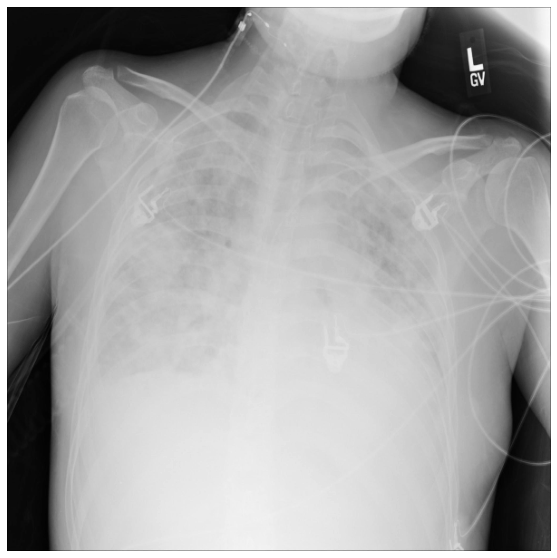
\includegraphics[width=3cm]{images/img.png}
		\caption{Original image}
		\label{fig:Stronger CLAHE}
	\end{subfigure}\hspace{12pt}
	\begin{subfigure}[c]{.4\linewidth}
		\centering
		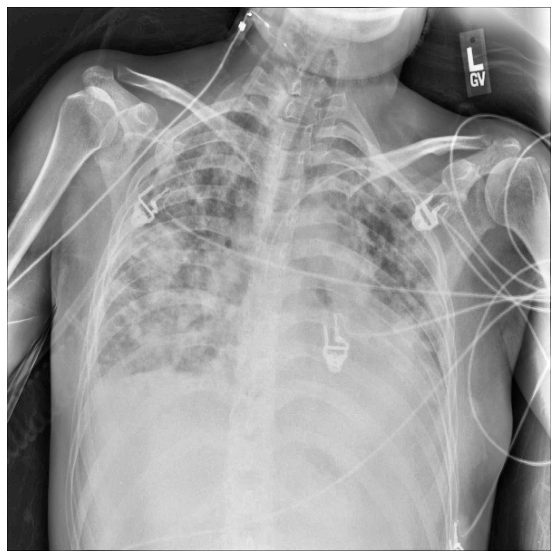
\includegraphics[width=3cm]{images/clahe.png}
		\caption{Clahe}
		\label{fig:tophat}
	\end{subfigure}\vspace{12pt}
	\caption{Original image and CLAHE}
	\label{fig:img}
\end{figure}

\newpage
\subsection{CNN}
The choice of the neural network is fundamental to create a stable and performing model.
Several families of networks are present in the literature, each with its own characteristics that are better suited for some types of tasks. 
    
As demonstrated by Ng et al. \cite{CHEXRAY} recently however, most of the models have been created to maximize performance on the Imagenet \cite {IMAGENET} problem, while today, the various deep learning works have focused on various types of different tasks, including medical tasks. As shown in the work carried out by Ng et al. \cite{CHEXRAY}, the network that perform best on the ChestXray dataset are the Inception networks that were not built on the basis of Imagenet. Furthermore, it is shown that even very small networks such as resnet18 achieve excellent results with the use of pretrained weights. The networks chosen by us for the comparison were: ResNet \cite{RESNET}, ResNest \cite{RESNEST}, Inception \cite{INCEPTION}, DenseNet \cite{DENSENET}, EfficientNetB2 \cite{EFFNET}.
Since our problem is similar to the CheXpert, We expect to get better results on those models, such as Inception, that are not based on ImageNet. We also believe that for this particular problem, a larger network could not be useful, leading to overfitting.
    
The test results are shown in Tables~V and Table~VI. As We can see, some models are not suitable for the problem in question, such as ResNest50, which only achieves an auc of 0.7. The choice of models was made with the following training procedure:
Epochs: 30
Early Stopping: 5 epochs if validation loss does not improve
Learning rate: 0.001 with a reduction of 0.4 after 3 epochs if the validation loss does not improve.
Pretrained weights: imagenet and noisy-student for efficientnetB2.
As We expected, also given the results obtained by Ng et al \cite{CHEXRAY}, the best neural network is EfficientNetB2 \cite{EFFNET}.
Once the best model was selected, We proceeded with training based on cross validation. We have selected 5 folds, using the split techniques discussed in the \ref{dataset} section

\subsection{Optimizers}
Since our approach is based on deep learning, it is important to choose the right loss function and the right optimizer to achieve the best possible performance. In this phase of our work, We proceeded incrementally, first choosing the CNN, then the optimizer, and finally the loss function. All the tests carried out to find the right loss and optimizer were carried out using the CNN that gave us the best results.
In recent years, with the advent of deep learning, more studies have focused on finding new optimizers. There are two main approaches, the first is based on the extension of the classic SGD \cite{SGD}, while the other approach is adaptive, and the most famous optimizers are Adam \cite{ADAM} and Adagrad \cite{ADAGRAD}. For image classification tasks, SGD has been shown to perform better in general, while adaptive optimizers like Adam are better at NLP problems. In recent studies, the surface of the loss function in image classification cases has begun to be better understood, and therefore new optimizers have been developed to be able to improve performance. Among all the optimizers present in the literature, We have chosen only 2 of them, AdaBound \cite{ADABOUND} and AdaBelief \cite{ADABELIEF}, since the approach used is to combine the strengths of SGD and Adam. 
Furthermore, as demonstrated by Chen et Kyrillidis \cite{DEMON}, another possible approach is to use decaying momentum and the performances on both Adam and SGD are better. 
So We decided to compare the SGD optimizers in the Decaying Momentum version, AdaBound, AdaBelief and Adam, tested both in the original version and in the version with Decaying Momentum. 

\subsection{Loss}
The task in question is a multilabel task, in which multiple labels can be present in a sample. The most used loss for this task is the Binary Cross Entropy. As mentioned in section 2, to try to stem the class imbalance problem, weights were calculated for each label and these weights were used in the loss function.
As for the optimizers, also for the loss functions, in recent years new functions have been proposed that are useful for the various machine learning tasks. Taking a cue from regression, in which penalty terms are used to improve the model's performance, We too have decided to test various versions of binary crossentropy using the main regularization techniques. Then, the BCE with L1, L2 and Elastic Net regularizer \cite{ELANET} were tested.

Furthermore, from a recent study by Liu et al. \cite {ELR}, a new loss function has been proposed for multiclassification problems with class imbalance. We have decided to adapt this function to the case of multi-label, to see if We can get a significant improvement on the overall results.

    
\section{Results}

\subsection{CNN}
The results obtained from our test shows that EfficientNetB2 is the best CNN suited for this task. This results is aligned with the results obtained in \cite{CHEXRAY}. Actually, if We look at the raw results obtained, the best performing net is EfficientNetB5, but since the difference is negligible, since the difference between the training and validation results is much smaller, meaning that EfficientNetB5 has overfitted the data, whilst EfficientNetB2 not. Also, We believe that a smaller net is best also for speed purposes, even if in this context, speed is not a critical requirement. 


\subsection{Optimizers}
From our results, We can clearly see that traditional methods such as SGD and Adam quickly converge to the minima, even though they are not so stable during the training process, leading to overfitting after few epochs. On the other hand, recent approaches like Adabound and Adabelief, in this case are slower to converge but they are really stable, and overfitting is not present in the early stages. From the results obtained, We decided to use Adam at first, since it converges quickly and leads us to good results after few epochs, and in a second stage We trained the model using Adabelief, since it works better when approaching the minima, as showed by Zhuang et al. The results obtained are shown in Table~VII and Table~VIII. 
    
\subsection{Loss}
From the results obtained from our test, We show that the weighted binary cross entropy loss, plus the L1 regularization, achieves better performance than the other losses proposed. In order to select the best loss function, We computed another metric, the AMCC. Taking inspiration from the AUC \cite{AUC}, We computed the Matthew Correlation Coefficient \cite{MCC} index curve at first, and then We computed the Area under the MCC curve, considering all the threshold in the range [0-1]. The MCC index is a measure of the quality of a binary classifier, and it differs from other metrics, such as F1 score or accuracy and recall, since it considers all the elements of the confusion matrix, making it a more robust index.
The BCE loss gives good results on AUC, but if We look at labels that are highly unbalanced, as ETT-Abnormal, the AMCC is close to 0, meaning that the classifier behaves as a random classifier.


The reason why We obtain such a high AUC score with BCE on these labels, it's because of the highly unbalance of the two classes, as show in \ref{dataset}, and so, even if the classifier outputs the same results for all the samples, the AUC can be still high. Our approach of adding some regularization by weighting the classes for each AUC and adding different kinds of penalization led us to achieve higher scores both on AUC and AMCC, with the jump on the AMCC being larger. The loss functions that achieves the highest performance is the BCE with L1 norm penalization. Indeed, with this function, both the AUC and AMCC are the highest among all the other losses tested.


The results obtained are present in Table~III and Table~IV. In most cases, the BCE with L1 regularization performs better than the others. Note the low performance of all the functions for the CVC labels. This type of catheter is therefore more difficult to classify, as there are a much greater number of samples than the other labels and it is therefore necessary to choose the best loss function for these three labels.
 
Another thing to see is the Early Learning Regularization Loss, that for this particular task, performs better than vanilla BCE, but the results are still lower than BCE + L1.

After running the tests on the loss function, We have finally built the model, and We took the highest performing model, and We applied a second stage training as described  earlier in this chapter.
After performing a 5-fold cross validation, the score obtained is 0.93.
The 5 folds used in this stage are computed as described in \ref{dataset}.


\section{Conclusion}
\subsection{Reliability of results}
Our results are satisfactory although they may seem, at first glance, lower than the highest scores in the top of the competition. However, there is an important consideration to be made in this regard:

Most kaggle users aim at winning the competition by getting the highest results, but this does not mean designing the model that generalize better on all the input data.
Most of them does not apply the techniques used by us that acts as regularizer:

\subsubsection{Lack of data preprocessing}
By feeding the data to the model without performing any preprocessing operations, the results obtained are very high. This is because the model simply does not learn to distinguish the different classes given the highly unbalanced distribution of the data. Specifically, this problem was partly demonstrated by us by comparing the BCE loss function with our weighted BCE loss function with the addition of regularization. Another thing to take into consideration is the size of the images. By feeding into the model small images, the model could learn to distinguish the classes not by taking into consideration the tubes.


\subsubsection{Dataset split and data leakage}
The presence of images that refer to the same patient, not present exclusively in the training or validation, results in a performance boost on the validation set which is not always true. Another factor to consider is the split of the dataset keeping the distribution of the datasets homogeneous between train and validation. The absence of even just one of these measures leads to unreliable results despite the score obtained.
\subsubsection{Noise not considered}
The addition of noise in the data augmentation makes the model more robust at the expense of performance that without this addition, at times, can be lower. Given the importance of the problem, We considered it more correct to build a robust model that is insensitive to noise in order to avoid attacks from adversarial models.\cite{NOISE} \cite{NOISE2}.

\subsection{Other experimented methods} 
In addition to the method presented in the previous sections, other methods have been tested, but have not led to the desired results.

\subsubsection{Different Image Preprocessing}
In addiction to CLAHE, We also tried other image preprocessing techniques. Out of all image preprocessing techniques applied, the one that gave us the best results was the one with just CLAHE. The other methods experimented are shown in Fig~\ref{fig:imageproc}.

\begin{figure}[H]
	\centering
	\begin{subfigure}[c]{.4\linewidth}
		\centering
		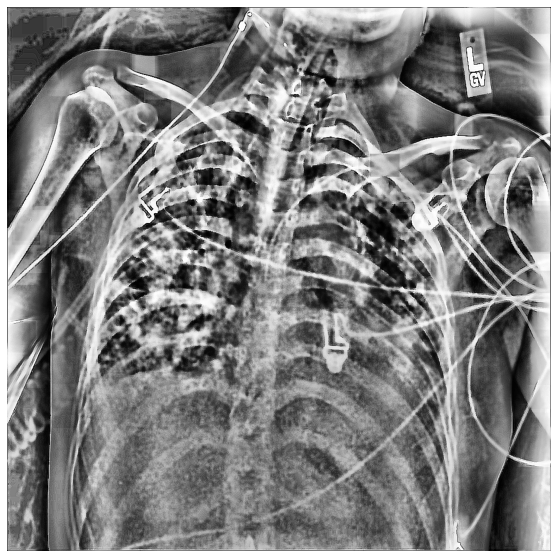
\includegraphics[width=3cm]{images/clahe2.png}
		\caption{Stronger CLAHE}
		\label{fig:Stronger CLAHE}
	\end{subfigure}\hspace{12pt}
	\begin{subfigure}[c]{.4\linewidth}
		\centering
		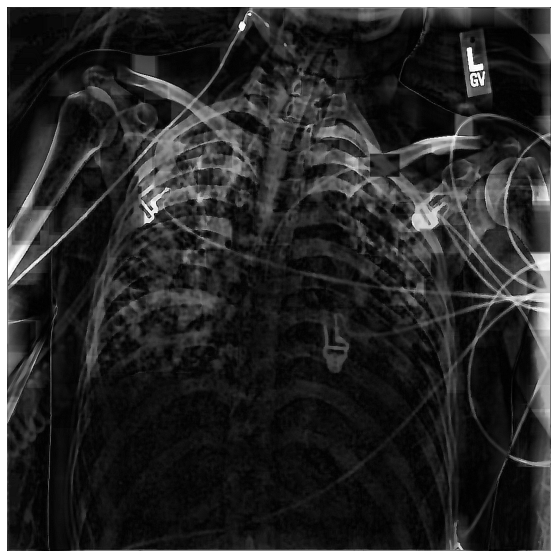
\includegraphics[width=3cm]{images/th.png}
		\caption{Top Hat}
		\label{fig:tophat}
	\end{subfigure}\vspace{12pt}
	\begin{subfigure}[c]{.4\linewidth}
		\centering
		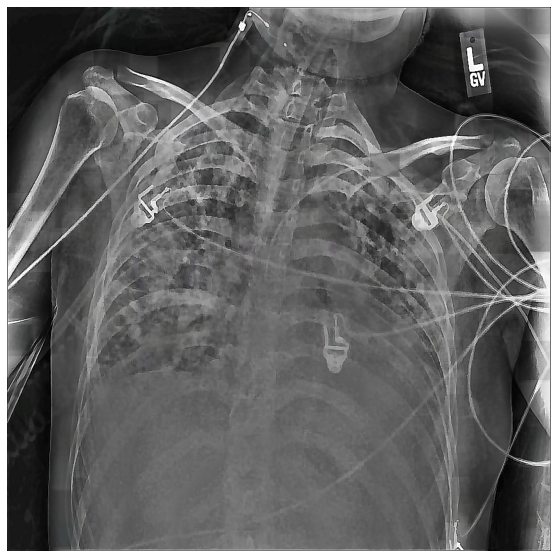
\includegraphics[width=3cm]{images/thcl.png}
		\caption{Top Hat + CLAHE}
		\label{fig:tophatclahe}
	\end{subfigure}\hspace{12pt}
	\begin{subfigure}[c]{.4\linewidth}
		\centering
		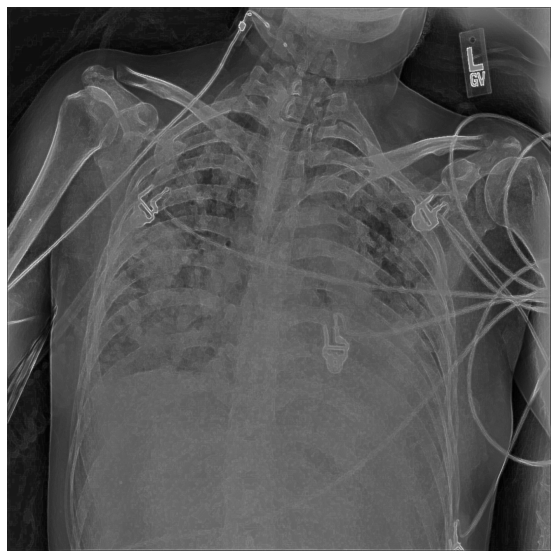
\includegraphics[width=3cm]{images/sobel.png}
		\caption{Sobel edges + CLAHE}
		\label{fig:sobel}
	\end{subfigure}
	\caption{Different Image processing.}
	\label{fig:imageproc}
\end{figure}


\subsubsection{Siamese network}
Another method tested is based on the use of the Siamese network and the annotations provided with the dataset. The basic idea was to create a hybrid between segmentation and distillation in which a Siamese network is used whose inputs are the original image and the corresponding mask image obtained thanks to annotations. The experimentation of this method is due to the fact that the computational resources available to us were very limited and therefore the use of segmentation was not possible. Following this first training, the Siamese net weights were transferred to the original model and a fine tuning was carried out. The results obtained, however, were slightly lower than those obtained without the use of this methodology which We consequently decided to put aside.

\subsubsection{Multihead}
Another approach tested is that of using multihead, a small part of independent networks, for each subset of labels. This approach can give better results because, by making the learning of one label group decoupled from the others, it can reduce variance and consequently overfitting. The label groups used were ETT, NGT, CVC, Swan-Ganz. The single head was composed as shown in Fig~\ref{fig:head}, taking inspiration from \cite{REPVGG}:
\begin{figure}[!hbt]
	\begin{center}
		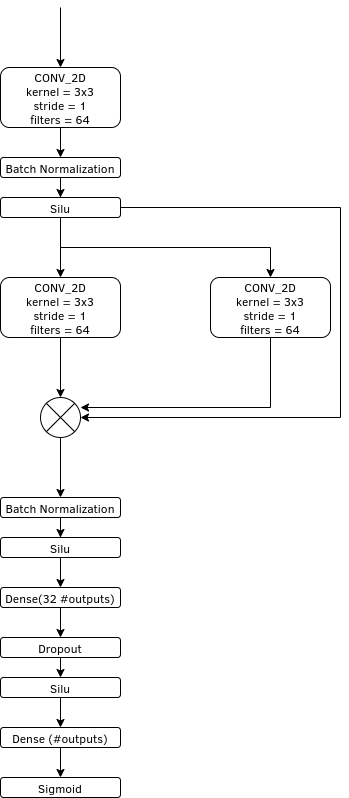
\includegraphics[scale=0.30]{images/head.png}
		\caption{Head model design}
		\label{fig:head}
	\end{center}
\end{figure}
	
However, the results obtained were lower than expected. By designing the network more accurately, better results could be obtained but this was not possible due to the limited time available.
\section{Future works}
As discussed in the previous paragraph, some alternative methodologies tested by us did not lead to the desired results. However, it is possible to consider more classical approaches such as distillation methods with teacher-student models or the use of segmentation

\subsection{Different Multihead}
An alternative to multihead is the approach whereby each group of labels uses a different network and, consequently, the weights of the networks are not shared. This method is an extreme extension of our concept of multihead which therefore, in theory, should lead to better results as each single network learns to classify only a group of classes that share the same features, unlike a method in which only one is used. network that must learn all the different features of the various labels.

\subsection{Segmentation}
Another approach is to use the annotations present in the dataset to create a segmentation model and use this result as an input for a classifier. This approach could not be as good as the others, since the annotations are only available to a third of the dataset. Other segmentation approaches are alrealdy present in literature, as this work by Chen et al\cite{SEGMENTATION}.

\subsection{Knowledge Distillation}
Another approach is to use distillation methods such as teacher-student models \cite{DISTILLATION}, using both the original dataset and also the annotation images. These models have been shown to improve the performance of the model, as shown Song et al. \cite{DISTILLATION2}. Here is a brief example of a distillation method in Fig~\ref{fig:teachstud}.

\begin{figure}[!hbt]
	\begin{center}
		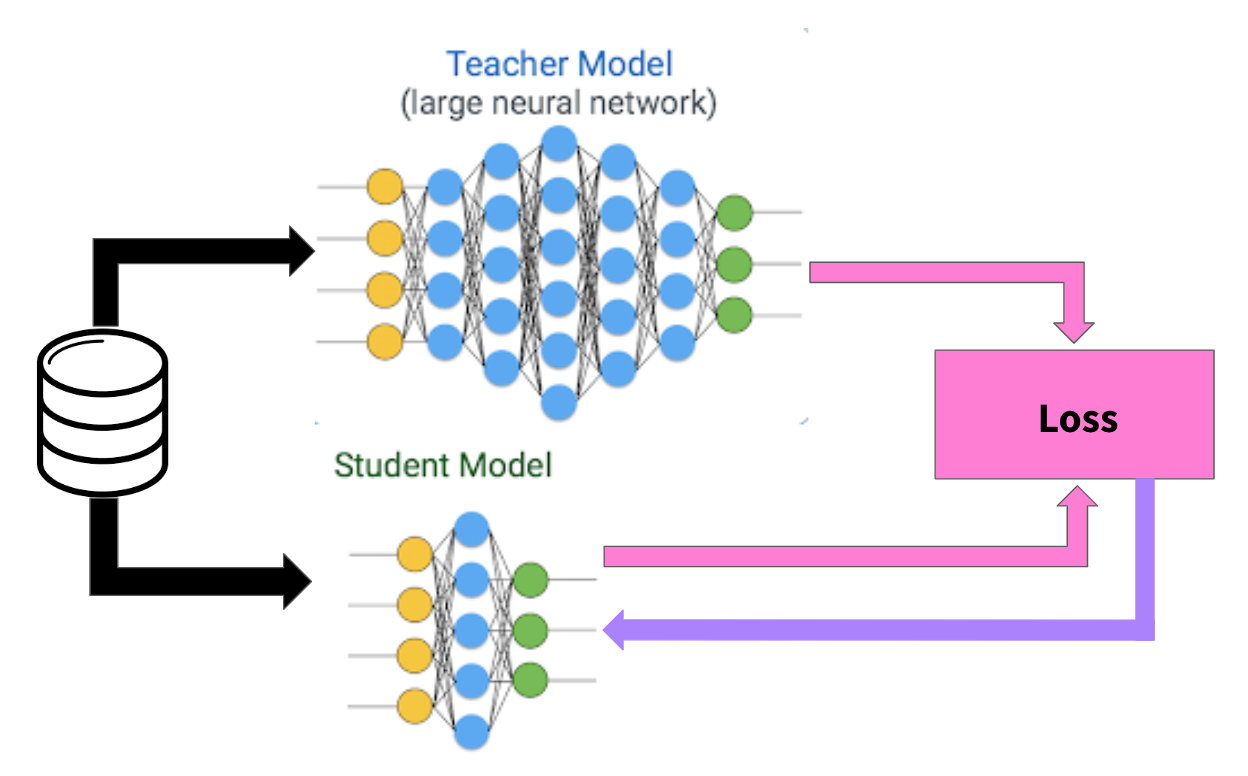
\includegraphics[scale=0.20]{images/distillation.png}
		\caption{Teacher student model}
		\label{fig:teachstud}
	\end{center}
\end{figure}

\clearpage
\begin{thebibliography}{5}
	\bibitem{RANZCR}
	RANZCR CLiP - Catheter and Line Position Challenge. 
	\url{https://www.kaggle.com/c/ranzcr-clip-catheter-line-classification}
				
	\bibitem{CLAHE}
	SS. M.~Pizer, R.~E.~Johnston, J.~P.~Ericksen, B.~C.~Yankaskas and K.~E.~Muller, "Contrast-limited adaptive histogram equalization: speed and effectiveness," [1990] Proceedings of the First Conference on Visualization in Biomedical Computing, pp. 337-345
	\url{http://www.cs.unc.edu/techreports/90-035.pdf}
			    
	\bibitem{CLAHE2}
	Lee H, Mansouri M, Tajmir S, Lev MH, Do S. A Deep-Learning System for Fully-Automated Peripherally Inserted Central Catheter (PICC) Tip Detection. J Digit Imaging. 2018;31(4):393-402.
			
	\bibitem{EFFNET}
	M.~Tan, Quoc V.~Le 
	EfficientNet: Rethinking Model Scaling for Convolutional Neural Networks
	\url{https://arxiv.org/pdf/1905.11946.pdf}
				
	\bibitem{SGD}
	J.~Kiefer and J.~Wolfowitz
	Stochastic Estimation of the Maximum of a Regression Function
	The Annals of Mathematical Statistics
	Vol. 23, No. 3 (Sep., 1952), pp. 462-466 (5 pages)
			
	\bibitem{ADAM} 
	Diederik P.~Kingma,     Jimmy Lei Ba
	Adam: A Method for Stochastic Optimization
	ICLR 2015
	\url{https://arxiv.org/pdf/1412.6980.pdf}
			    
	\bibitem{ADAGRAD} 
	R.~Anil, V.~Gupta, T.~Koren, Y.~Singer
	Memory-Efficient Adaptive Optimization
	\url{https://arxiv.org/pdf/1901.11150.pdf}
			    
			    
	\bibitem{ADABOUND}
	L.~Luo, Y.~Xiong, Y.~Liu, Xu Sun
	Adaptive gradient methods with dynamic bound of learning rate
	ICLR 2019
	\url{https://arxiv.org/pdf/1902.09843.pdf}
			    
			    
	\bibitem{ADABELIEF}
	J.~Zhuang,T.~Tang,S.~Tatikonda,N.~Dvornek,Y.~Ding,X~Papademetris, J.~S.~Duncan
	AdaBelief Optimizer: Adapting Stepsizes by the Belief in Observed Gradients
	\url{https://arxiv.org/pdf/2010.07468v1.pdf}
			    
			    
	\bibitem{DEMON}
	J.~Chen, A.~Kyrillidis
	Decaying momentum helps neural network training
	\url{https://arxiv.org/pdf/1910.04952v1.pdf}
			    
			    
	\bibitem{ELANET}
	H.~Zou, T.~Hastie
	Regularization and variable selection via the elastic net
	Journal of the Royal Statistical Society Series B
	Volume 67, Issue 2, Pages 301-320. April 2005
	\url{ https://doi.org/10.1111/j.1467-9868.2005.00503.x}
			    
			    
	\bibitem{ELR}
	S.~Liu, J.~N.-Weed, N.~Razavian, C.~Fernandez-Granda
	Early-Learning Regularization Prevents Memorization of Noisy Labels
	\url{https://arxiv.org/pdf/2007.00151.pdf}
			    
			    
	\bibitem{CHEXRAY}
	A.~Ke, W.~Ellsworth, O.~Banerjee, A.~Y..~Ng, P.~Rajpurkar
	CheXtransfer: Performance and Parameter Efficiency of ImageNet Models for Chest X-Ray Interpretation
	\url{https://arxiv.org/pdf/2101.06871.pdf}
			    
			    
	\bibitem{IMAGENET}
	J.~Deng, W.~Dong, R.~Socher, L.~Li, Kai~Li and Li~Fei-Fei, "ImageNet: A large-scale hierarchical image database," 2009 IEEE Conference on Computer Vision and Pattern Recognition, Miami, FL, USA, 2009, pp. 248-255
	\url{http://image-net.org/papers/imagenet_cvpr09.pdf}
			    
	\bibitem{RESNET}
	K.~He, X.~Zhang, S.~Ren, J.~Sun
	Deep Residual Learning for Image Recognition
	\url{https://arxiv.org/pdf/1512.03385.pdf}
			    
			    
	\bibitem{RESNEST}
	H.~Zhang, C.~Wu, Z.~Zhang, Y.~Zhu, H.~Lin, Z.~Zhang,Y.~Sun, T.~He, J.~Mueller, R.~Manmatha, Mu Li, A.~Smola
	ResNeSt: Split-Attention Networks
	\url{https://arxiv.org/pdf/2004.08955.pdf}
			    
			    
	\bibitem{DENSENET}
	G.~, Z.~Liu, K.~Q.~Weinberger, L.~van der Maaten
	Densely Connected Convolutional Networks
	\url{https://arxiv.org/pdf/1608.06993v3.pdf}
			    
			    
	\bibitem{INCEPTION}
	C. Szegedy et al., "Going deeper with convolutions," 2015 IEEE Conference on Computer Vision and Pattern Recognition (CVPR), Boston, MA, USA, 2015, pp. 1-9
	\url{https://arxiv.org/pdf/1409.4842v1.pdf}
	    
	\bibitem{MCC}
	Matthews B. W. (1975). Comparison of the predicted and observed secondary structure of T4 phage lysozyme. Biochimica et biophysica acta, 405(2), 442–451. https://doi.org/10.1016/0005-2795(75)90109-9
			    
			    
	\bibitem{AUC}
	Andrew P. Bradley,The use of the area under the ROC curve in the evaluation of machine learning algorithms,Pattern Recognition,Volume 30, Issue 7,1997,Pages 1145-1159,ISSN 0031-3203,
	https://doi.org/10.1016/S0031-3203(96)00142-2.
			
			    
	\bibitem{LEAK}
	Kaufman, Shachar & Rosset, Saharon & Perlich, Claudia. (2011). Leakage in Data Mining: Formulation, Detection, and Avoidance. Proceedings of the ACM SIGKDD International Conference on Knowledge Discovery and Data Mining. 6. 556-563.
	\url{https://doi.org/10.1145/2020408.2020496}
			    
			    
	\bibitem{SIAMESE}
	Chicco D. (2021) Siamese Neural Networks: An Overview. In: Cartwright H. (eds) Artificial Neural Networks. Methods in Molecular Biology, vol 2190. Humana, New York, NY. 
	\url{https://doi.org/10.1007/978-1-0716-0826-5_3}
			    
			    
	\bibitem{DISTILLATION}
	Z.~Che, S.~Purushotham, R.~Khemani, Y.~Liu
	Distilling Knowledge from Deep Networks with Applications to Healthcare Domain
	\url{https://arxiv.org/pdf/1512.03542.pdf}
			    
			    
	\bibitem{NOISE}
	Z.~You, J.~Ye, K.~Li, Z.~Xu, P.~Wang
	Adversarial Noise Layer: Regularize Neural Network By Adding Noise
	\url{https://arxiv.org/pdf/1805.08000.pdf}
			    
			    
	\bibitem{NOISE2}
	J.~Jin, A.~Dundar, E.~Culurciello
	Robust Convolutional Neural Networks under Adversarial Noise
	\url{https://arxiv.org/pdf/1511.06306.pdf}
		
		
	\bibitem{REPVGG}
	X.~Ding, X.~Zhang, N.~Ma, J.~Han, G.~Ding, J.~Sun
	RepVGG: Making VGG-style ConvNets Great Again
	\url{https://arxiv.org/pdf/2101.03697v1.pdf}
		
	\bibitem{DISTILLATION2}
	X.~Song, F.~Feng, X.~Han, X.~Yang, W.~Liu, L.~Nie
	Neural Compatibility Modeling with Attentive Knowledge Distillation
	\url{https://arxiv.org/pdf/1805.00313.pdf}
	
	\bibitem{SEGMENTATION}
	H.~Chen,S.~Ruan,S.~Huang, Y.~Peng
	Lung X-ray Segmentation using Deep Convolutional Neural Networks on Contrast-Enhanced Binarized Images
	\url{https://doi.org/10.3390/math8040545}
	
			
\end{thebibliography}

\clearpage

\begin{table}[ht]
	\centering
	\begin{minipage}{\linewidth}
		\centering
		\begin{tabular}{||l c c c c c c c c c c c c||}
			\hline
			Loss     & ETT Abn & ETT Brd & ETT   & NGT Abn & NGT Brd & NGT Inc.Img & NGT   & CVC Abn & CVC Brd & CVC   & S.G.  & Mean  \\ [0.5ex] \hline\hline
			BCE      & 0.014   & 0.207   & 0.85  & 0.008   & 0.041   & 0.56        & 0.701 & 0.36    & 0.309   & 0.439 & 0.867 & 0.396 \\ \hline
			WBCE     & 0.176   & 0.332   & 0.85  & 0.157   & 0.187   & 0.539       & 0.64  & 0.289   & 0.282   & 0.398 & 0.467 & 0.392 \\ \hline
			BCE L1   & 0.282   & 0.39    & 0.873 & 0.189   & 0.26    & 0.637       & 0.727 & 0.395   & 0.354   & 0.483 & 0.869 & 0.496 \\ \hline
			BCE L2   & 0.014   & 0.101   & 0.724 & 0.049   & 0.062   & 0.415       & 0.41  & 0.016   & 0.027   & 0.026 & 0.567 & 0.219 \\ \hline
			BCE L1L2 & 0.017   & 0.132   & 0.784 & 0.017   & 0.054   & 0.407       & 0.6   & 0.021   & 0.03    & 0.031 & 0.557 & 0.241 \\ \hline
			WELR     & 0.152   & 0.326   & 0.849 & 0.153   & 0.218   & 0.588       & 0.692 & 0.315   & 0.311   & 0.436 & 0.852 & 0.445 \\ \hline
			FOCAL    & 0.02    & 0.152   & 0.696 & 0.03    & 0.054   & 0.316       & 0.355 & 0.114   & 0.044   & 0.057 & 0.568 & 0.219 \\ [0.5ex] \hline
		\end{tabular}
		\label{tab:loss_amcc}
		\caption{Losses Area MCC validation set}
	\end{minipage}
			  
	\bigskip
	\begin{minipage}{\linewidth}
		\centering
		\begin{tabular}{||l c c c c c c c c c c c c||}
			\hline
			Loss     & ETT Abn & ETT Brd & ETT   & NGT Abn & NGT Brd & NGT Inc.Img & NGT   & CVC Abn & CVC Brd & CVC   & S.G.  & Mean  \\ [0.5ex] \hline\hline
			BCE      & 0.95    & 0.946   & 0.99  & 0.883   & 0.921   & 0.972       & 0.976 & 0.848   & 0.809   & 0.86  & 0.994 & 0.913 \\ \hline
			WBCE     & 0.964   & 0.943   & 0.988 & 0.899   & 0.911   & 0.966       & 0.968 & 0.842   & 0.789   & 0.851 & 0.995 & 0.92  \\ \hline
			BCE L1   & 0.974   & 0.959   & 0.989 & 0.921   & 0.934   & 0.973       & 0.977 & 0.863   & 0.803   & 0.859 & 1.0   & 0.929 \\ \hline
			BCE L2   & 0.842   & 0.906   & 0.985 & 0.809   & 0.807   & 0.941       & 0.914 & 0.578   & 0.573   & 0.534 & 0.951 & 0.803 \\ \hline
			BCE L1L2 & 0.876   & 0.913   & 0.983 & 0.812   & 0.901   & 0.955       & 0.958 & 0.582   & 0.555   & 0.548 & 0.988 & 0.825 \\ \hline
			WELR     & 0.961   & 0.941   & 0.986 & 0.901   & 0.925   & 0.972       & 0.973 & 0.84    & 0.794   & 0.853 & 0.995 & 0.922 \\ \hline 
			FOCAL    & 0.92    & 0.937   & 0.988 & 0.849   & 0.883   & 0.958       & 0.961 & 0.689   & 0.619   & 0.629 & 0.985 & 0.856 \\ [0.5ex] \hline
		\end{tabular}
		\label{tab:loss_auc}
		\caption{Losses AUC validation set}
	\end{minipage}
			  
	\bigskip
	\begin{minipage}{\linewidth}
		\centering
		\begin{tabular}{||l c c c c c c c c c c c c||}
			\hline
			Models         & ETT Abn & ETT Brd & ETT   & NGT Abn & NGT Brd & NGT Inc.Img & NGT   & CVC Abn & CVC Brd & CVC   & S.G.  & Mean  \\ [0.5ex] \hline\hline
			InceptionV3    & 0.923   & 0.942   & 0.989 & 0.906   & 0.908   & 0.963       & 0.97  & 0.863   & 0.785   & 0.866 & 0.995 & 0.91  \\ \hline
			Resnet18       & 0.944   & 0.935   & 0.989 & 0.878   & 0.917   & 0.967       & 0.972 & 0.816   & 0.787   & 0.83  & 0.987 & 0.905 \\ \hline
			Densenet169    & 0.829   & 0.919   & 0.978 & 0.868   & 0.885   & 0.949       & 0.956 & 0.816   & 0.77    & 0.824 & 0.996 & 0.891 \\ \hline
			ResNest50      & 0.877   & 0.876   & 0.948 & 0.853   & 0.833   & 0.9         & 0.919 & 0.557   & 0.523   & 0.531 & 0.875 & 0.791 \\ \hline
			Resnet101      & 0.918   & 0.935   & 0.989 & 0.842   & 0.898   & 0.961       & 0.963 & 0.785   & 0.751   & 0.811 & 0.984 & 0.892 \\ \hline
			Xception       & 0.907   & 0.943   & 0.987 & 0.863   & 0.884   & 0.959       & 0.972 & 0.848   & 0.771   & 0.849 & 0.998 & 0.904 \\ \hline
			EfficientNetB2 & 0.924   & 0.952   & 0.99  & 0.894   & 0.936   & 0.973       & 0.979 & 0.858   & 0.814   & 0.878 & 0.992 & 0.921 \\ \hline
			EfficientNetB5 & 0.977   & 0.959   & 0.99  & 0.884   & 0.916   & 0.975       & 0.977 & 0.854   & 0.804   & 0.87  & 0.987 & 0.924 \\ [0.5ex] \hline
		\end{tabular}
		\label{tab:models_auc}
		\caption{Models AUC validation set}
	\end{minipage}
			  
	\bigskip
	\begin{minipage}{\linewidth}
		\centering
		\begin{tabular}{||l c c c c c c c c c c c c||}
			\hline
			Models         & ETT Abn & ETT Brd & ETT   & NGT Abn & NGT Brd & NGT Inc.Img & NGT   & CVC Abn & CVC Brd & CVC   & S.G.  & Mean  \\ [0.5ex] \hline\hline
			InceptionV3    & 0.052   & 0.408   & 0.85  & 0.031   & 0.117   & 0.599       & 0.682 & 0.426   & 0.339   & 0.508 & 0.903 & 0.447 \\ \hline
			Resnet18       & 0.004   & 0.159   & 0.837 & 0.019   & 0.046   & 0.455       & 0.647 & 0.209   & 0.29    & 0.379 & 0.749 & 0.345 \\ \hline
			Densenet169    & 0.004   & 0.139   & 0.741 & 0.01    & 0.044   & 0.465       & 0.453 & 0.284   & 0.226   & 0.326 & 0.663 & 0.305 \\ \hline
			ResNest50      & 0.001   & 0.045   & 0.546 & 0.007   & 0.009   & 0.164       & 0.271 & 0.005   & 0.004   & 0.007 & 0.043 & 0.1   \\ \hline
			Resnet101      & 0.006   & 0.114   & 0.794 & 0.007   & 0.064   & 0.473       & 0.587 & 0.149   & 0.158   & 0.294 & 0.735 & 0.307 \\ \hline
			Xception       & 0.008   & 0.163   & 0.801 & 0.018   & 0.054   & 0.522       & 0.656 & 0.333   & 0.219   & 0.377 & 0.824 & 0.361 \\ \hline
			EfficientNetB2 & 0.082   & 0.329   & 0.869 & 0.025   & 0.107   & 0.606       & 0.727 & 0.384   & 0.319   & 0.5   & 0.936 & 0.444 \\ \hline
			EfficientNetB5 & 0.012   & 0.295   & 0.864 & 0.016   & 0.053   & 0.597       & 0.678 & 0.379   & 0.296   & 0.483 & 0.895 & 0.415 \\ [0.5ex] \hline
		\end{tabular}
		\label{tab:models_amcc}
		\caption{Models Area MCC validation set}
	\end{minipage}
			  
	\bigskip
	\begin{minipage}{\linewidth}
		\centering
		\begin{tabular}{||l c c c c c c c c c c c c||}
			\hline
			Optmizer  & ETT Abn & ETT Brd & ETT   & NGT Abn & NGT Brd & NGT Inc.Img & NGT   & CVC Abn & CVC Brd & CVC   & S.G.  & Mean  \\ [0.5ex] \hline\hline
			AdaBelief & 0.008   & 0.196   & 0.856 & 0.006   & 0.036   & 0.511       & 0.637 & 0.262   & 0.242   & 0.389 & 0.801 & 0.359 \\ \hline
			Adam      & 0.001   & 0.092   & 0.71  & 0.005   & 0.015   & 0.434       & 0.539 & 0.028   & 0.054   & 0.055 & 0.508 & 0.222 \\ \hline
			DemonAdam & 0.004   & 0.13    & 0.832 & 0.019   & 0.085   & 0.526       & 0.581 & 0.131   & 0.047   & 0.072 & 0.797 & 0.293 \\ \hline
			AdaBound  & 0.001   & 0.132   & 0.831 & 0.005   & 0.016   & 0.517       & 0.639 & 0.189   & 0.221   & 0.368 & 0.755 & 0.334 \\ \hline
			DemonSGD  & 0.001   & 0.117   & 0.811 & 0.003   & 0.012   & 0.429       & 0.572 & 0.025   & 0.06    & 0.056 & 0.177 & 0.206 \\ [0.5ex] \hline
		\end{tabular}
		\label{tab:optimizers_amcc}
		\caption{Optimizers Area MCC validation set}
	\end{minipage}
			  
	\bigskip
	\begin{minipage}{\linewidth}
		\centering
		\begin{tabular}{||l c c c c c c c c c c c c||}
			\hline
			Optmizer  & ETT Abn & ETT Brd & ETT   & NGT Abn & NGT Brd & NGT Inc.Img & NGT   & CVC Abn & CVC Brd & CVC   & S.G.  & Mean  \\ [0.5ex] \hline\hline
			AdaBelief & 0.942   & 0.942   & 0.989 & 0.833   & 0.9     & 0.956       & 0.965 & 0.806   & 0.76    & 0.817 & 0.992 & 0.89  \\ \hline
			Adam      & 0.895   & 0.945   & 0.988 & 0.866   & 0.902   & 0.961       & 0.966 & 0.672   & 0.651   & 0.675 & 0.993 & 0.864 \\ \hline
			DemonAdam & 0.95    & 0.934   & 0.988 & 0.887   & 0.913   & 0.973       & 0.97  & 0.621   & 0.566   & 0.591 & 0.983 & 0.845 \\ \hline
			AdaBound  & 0.893   & 0.933   & 0.987 & 0.824   & 0.878   & 0.959       & 0.966 & 0.796   & 0.743   & 0.811 & 0.991 & 0.879 \\ \hline
			DemonSGD  & 0.891   & 0.924   & 0.985 & 0.83    & 0.866   & 0.954       & 0.957 & 0.627   & 0.611   & 0.605 & 0.939 & 0.832 \\ [0.5ex] \hline
		\end{tabular}
		\label{tab:optimizers_auc}
		\caption{Optimizers AUC validation set}
	\end{minipage}
\end{table}

\end{document}